\section{Disassembler Demonstration}
\Cref{fig:s1asm} shows a sample program i.e. "\textit{1's COMPLEMENT OF A 16-BIT NUMBER}" loaded in the assembly language editor. It is then assembled by pressing the \textbf{Assemble} button. After assembling, memory content  and assembler workspace are shown in \cref{fig:s1asmMem} and \cref{fig:s1asmWork} respectively. Then the \textbf{Hexcode} is saved by selecting "FILE$ \rightarrow $Save Hexcode" or presing "ALT+S". \\

The generated hexcode is now loaded in the Disassembler editor by selecting "FILE$ \rightarrow $Load Hexcode" or presing "ALT+O". As it can be seen in \cref{fig:s1hex} the Intel Hex formatted code is syntactically highlighted.
Now, press the \textbf{Disassemble}. If there is some error in the code that line will be highlighted in red.  The tabbed window will not automatically change, even if there is no error. Now open the assembler editor the code is disassembled, as given in \cref{fig:s1dis}. Simultaneously the memory content is also loaded which is same as shown in \cref{fig:s1asmMem}. But, it is to be remembered that assembler workspace will remain empty, until the code is assembled from the assembler editor.  

\begin{figure}[htbp]
        \centering
        \begin{subfigure}[b]{0.4\textwidth}
                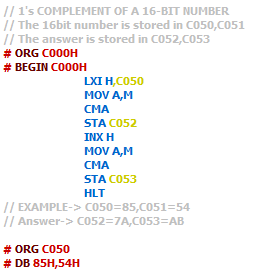
\includegraphics[width=\textwidth]{sampleCode1}
                \caption{Assembled Code}
                \label{fig:s1asm}
        \end{subfigure}
       \begin{subfigure}[b]{0.3\textwidth}
                       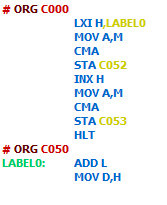
\includegraphics[width=\textwidth]{sampleCode1Rev}
                       \caption{Disassembled Code}
                       \label{fig:s1dis}
               \end{subfigure}
		\\        \vspace{20pt}
       \begin{subfigure}[b]{0.5\textwidth}
                       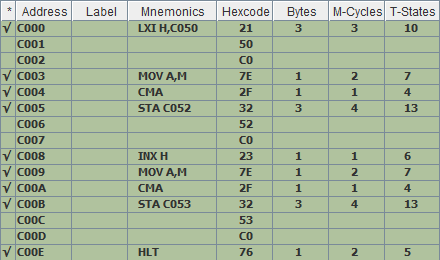
\includegraphics[width=\textwidth]{sampleCode1Asm}
                       \caption{Assembler Workspace after Assembling}
                       \label{fig:s1asmWork}
               \end{subfigure}
       \begin{subfigure}[b]{0.4\textwidth}
                       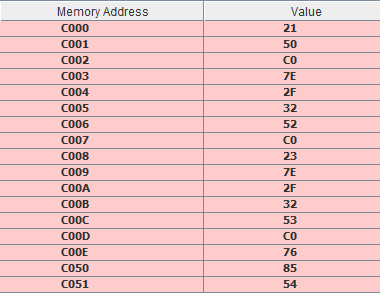
\includegraphics[width=\textwidth]{sampleCode1Mem}
                       \caption{Memory Content after Assembling}
                       \label{fig:s1asmMem}
               \end{subfigure}    
		\\        \vspace{20pt}
       \begin{subfigure}[b]{0.5\textwidth}
                       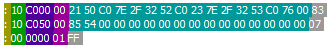
\includegraphics[width=\textwidth]{sampleCode1Hex}
                       \caption{Hexcode of Assembled code}
                       \label{fig:s1hex}
               \end{subfigure}    
         \\ \vspace{20pt}          
   \caption{Showing working of Disassembler}
\end{figure}